% -*- mode: latex; -*- mustache tags:  
\documentclass[10pt,twoside,english]{_support/latex/sbabook/sbabook}
\let\wholebook=\relax

\usepackage{import}
\subimport{_support/latex/}{common.tex}

%=================================================================
% Debug packages for page layout and overfull lines
% Remove the showtrims document option before printing
\ifshowtrims
  \usepackage{showframe}
  \usepackage[color=magenta,width=5mm]{_support/latex/overcolored}
\fi


% =================================================================
\title{Concurrent Programming in Pharo}
\author{Stéphane Ducasse and Guillermo Polito}
\series{The Pharo Technology Booklet Collection — edited by S. Ducasse}

\hypersetup{
  pdftitle = {Concurrent Programming in Pharo},
  pdfauthor = {Stéphane Ducasse and Guillermo Polito},
  pdfkeywords = {concurrence, task, thread, semaphore, Pharo, Smalltalk}
}


% =================================================================
\begin{document}

% Title page and colophon on verso
\maketitle
\pagestyle{titlingpage}
\thispagestyle{titlingpage} % \pagestyle does not work on the first one…

\cleartoverso
{\small

  Copyright 2017 by Stéphane Ducasse and Guillermo Polito.

  The contents of this book are protected under the Creative Commons
  Attribution-ShareAlike 3.0 Unported license.

  You are \textbf{free}:
  \begin{itemize}
  \item to \textbf{Share}: to copy, distribute and transmit the work,
  \item to \textbf{Remix}: to adapt the work,
  \end{itemize}

  Under the following conditions:
  \begin{description}
  \item[Attribution.] You must attribute the work in the manner specified by the
    author or licensor (but not in any way that suggests that they endorse you
    or your use of the work).
  \item[Share Alike.] If you alter, transform, or build upon this work, you may
    distribute the resulting work only under the same, similar or a compatible
    license.
  \end{description}

  For any reuse or distribution, you must make clear to others the
  license terms of this work. The best way to do this is with a link to
  this web page: \\
  \url{http://creativecommons.org/licenses/by-sa/3.0/}

  Any of the above conditions can be waived if you get permission from
  the copyright holder. Nothing in this license impairs or restricts the
  author's moral rights.

  \begin{center}
    
\includegraphics[width=0.2\textwidth]{_support/latex/sbabook/CreativeCommons-BY-SA.pdf}
  \end{center}

  Your fair dealing and other rights are in no way affected by the
  above. This is a human-readable summary of the Legal Code (the full
  license): \\
  \url{http://creativecommons.org/licenses/by-sa/3.0/legalcode}

  \vfill

  % Publication info would go here (publisher, ISBN, cover design…)
  Layout and typography based on the \textcode{sbabook} \LaTeX{} class by Damien
  Pollet.
}


\frontmatter
\pagestyle{plain}

\tableofcontents*
\clearpage\listoffigures

\mainmatter


This book describes the low-level abstractions available in Pharo for concurrent programming. 
It explains pedagogically different aspects. 
Now, if you happen to create many green threads (called Process in Pharo) we suggest that you 
have a look at TaskIt. TaskIt is an extensible library to manage concurrent processing at a higher-level of abstractions. 
You should definitively have a look at it. 
\chapter{Concurrent Programming in Pharo}
Pharo is a sequential language since at one point in time there is only one computation carried on. However, it has the ability to run programs concurrently by interleaving their executions. The idea behind Pharo is to propose a complete OS and as such a Pharo run-time offers the possibility to execute different processes in Pharo lingua (or green threads in other languages) that are scheduled by a process scheduler defined within the language.

Pharo's concurrency is \textit{collaborative} and \textit{preemptive}. It is \textit{preemptive} because a process with higher priority can interrupt the current running one. It is \textit{collaborative} because the current process should explicitly release the control to give a chance to the other processes of the same priority to get executed by the scheduler.

In this chapter we present how processes are created and their lifetime. We present
semaphores since they are the most basic building blocks to support concurrent programming and the infrastructure to execute concurrent programs. We will show how the process scheduler manages the system. 

In a subsequent chapter we will present the other abstractions: Mutex, Monitor and Delay.
\section{Studying an example}
Pharo supports the concurrent execution of multiple programs using independent processes (green threads). 
These processes are lightweight processes as they share a common memory space. 
Such processes are instances of the class \textcode{Process}. 
Note that in operating systems, processes have their own memory and communicate via pipes supporting a strong isolation. 
In Pharo, processes are what is usually called a (green) thread in other languages. 
They have their own execution flow but share the same memory space and use concurrent abstractions such semaphores to synchronize with each other.
\section{A simple example}
Let us start with a simple example. 
We will explain all the details in subsequent sections. 
The following code creates two processes using the message \textcode{fork} sent to a block. 
In each process we enumerate numbers. 
During each loop step, using the expression \textcode{Processor yield}, the current process stops its execution to give a chance to other processes with the same priority to get executed. 
At the end of the loop we refresh the \textcode{Transcript} output.

\begin{displaycode}{plain}
[ 1 to: 10 do: [ :i |
  Transcript nextPutAll: i printString, ' '.
  Processor yield ].
Transcript endEntry ] fork.

[ 101 to: 110 do: [ :i |
  Transcript nextPutAll: i  printString, ' '.
  Processor yield ].
Transcript endEntry ] fork
\end{displaycode}

Figure \ref{TwoInterleavingProcesses} shows the output produced by the execution of the snippet.


\begin{figure}

\begin{center}
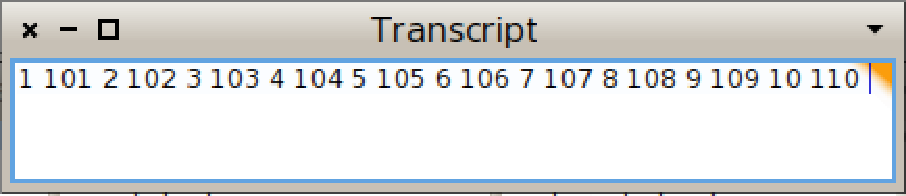
\includegraphics[width=0.6\textwidth]{/Users/ducasse/Workspace/FirstCircle/MyBooks/Bk-Writing/PharoBooks2/Booklet-ConcurrentProgramming/_result/pdf/Chapters/figures/TwoInterleavedProcesses.pdf}\caption{Two interleaving processes.\label{TwoInterleavingProcesses}}\end{center}
\end{figure}


We see that the two programs run concurrently, each outputting a number at a time and not producing two numbers in a row.

Let us look at what is a process.
\section{Process Lifetime}
A process can be in different states depending on its life-time (\textbf{runnable}, \textbf{suspended}, \textbf{executing}, \textbf{waiting}, \textbf{terminated}) as shown in Figure \ref{processStates}. We look at such states now.


\begin{figure}

\begin{center}
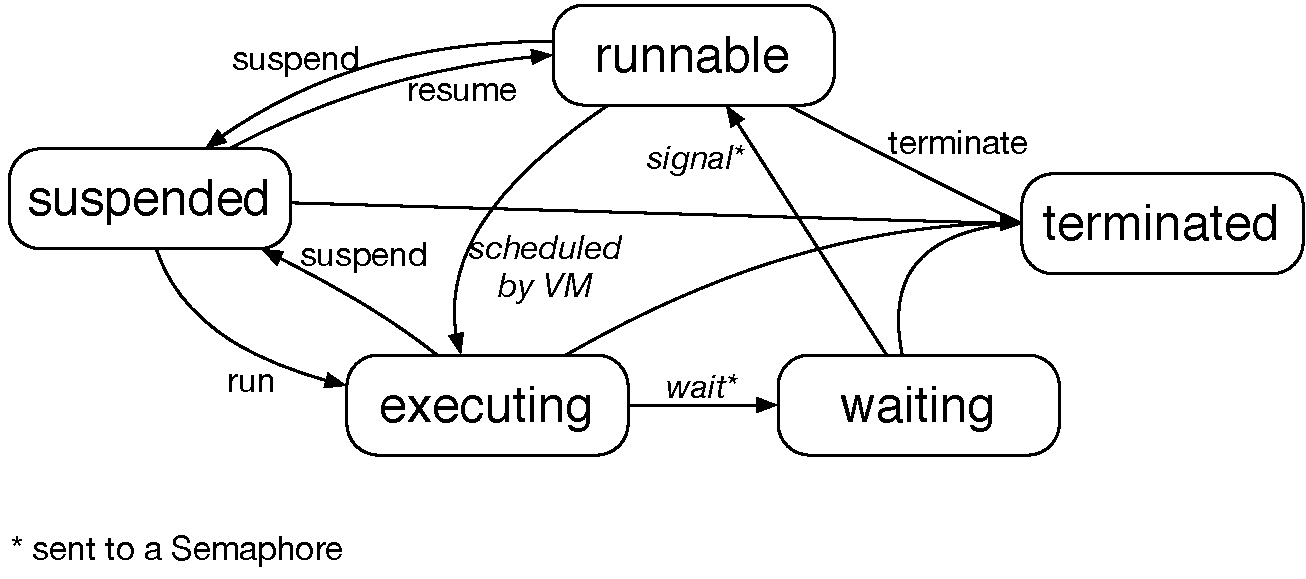
\includegraphics[width=1.0\textwidth]{/Users/ducasse/Workspace/FirstCircle/MyBooks/Bk-Writing/PharoBooks2/Booklet-ConcurrentProgramming/_result/pdf/Chapters/figures/processStates.pdf}\caption{Process states:  A process (green thread) can be in one of the following states: \textbf{runnable}, \textbf{suspended}, \textbf{executing}, \textbf{waiting}, \textbf{terminated}.\label{processStates}}\end{center}
\end{figure}

\subsection{Creating and launching a new process}
To execute concurrently a program, we write such a program in a block and send to the block the message \textcode{fork}.

\begin{displaycode}{plain}
[ 1 to: 10 do: [ :i | i  printString traceCr ] 
	] fork
\end{displaycode}

This expression creates an instance of the class \textcode{Process}. 
It is added to the list of scheduled processes of the process scheduler (as we will explained later). 
We say that this process is \textcode{runnable}: 
it can be potentially executed. 
It will be executed when the process scheduler will schedule it as the current running process and give it the flow of control.
At this moment the block of this process will be executed.
\subsection{Creating a process without scheduling it}
We can also create a process which is not scheduled (hence \textbf{suspended}) using the message \textcode{newProcess}.

You can i

\begin{displaycode}{plain}
| pr |
pr := [ 1 to: 10 do: [ :i |
   i  printString traceCr ] ] newProcess.
pr inspect
\end{displaycode}

This creates a process in \textcode{suspended} state, it is not added to the list of the scheduled processes of the process scheduler. 
It is not that is not \textcode{runnable}. It can be scheduled sending it the message \textcode{resume}.

In the inspector open by the previous expression, you can execute \textcode{self resume} and then the process will be scheduled. 

\begin{displaycode}{plain}
self resume
\end{displaycode}

Also \textbf{suspended} process can be executed immediately by sending it the \textcode{run} message.
The message \textcode{run} suspends the current process and execute the receiver process at the highest priority.
\subsection{Passing arguments to a process}
You can also pass arguments to a process with the message \textcode{newProcessWith: anArray} as follows:

\begin{displaycode}{plain}
| pr |
pr := [ :max |
  1 to: max do: [ :i |
    i  printString crLog ] ] newProcessWith: #(20).
pr resume
\end{displaycode}

Note that the elements of the argument array are passed to the corresponding block parameters.
\subsection{Suspending and terminating a process}
A process can also be temporarily suspended (i.e., stopped) using the message \textcode{suspend}. 
A suspended processed can be rescheduled using the message \textcode{resume}. 
We can also terminate a process using the message \textcode{terminate}. 
A terminated process cannot be scheduled any more.
\subsection{Creating a waiting process}
As you see on Figure \ref{processStates} a process can be in a waiting state.
It means that the process is blocked waiting to be rescheduled. 
This happens when you need to synchronize concurrent processes.
The basic synchronization mechanism is a semaphore and we will cover this deeply in subsequent sections.
\section{Creation API Summary}
The process creation API is composed of messages sent to blocks. 

\begin{itemize}
\item \textcode{{[} {]} newProcess} creates a unscheduled process whose code is the receiver bloc. The priority is the one of the active process. 
\item \textcode{{[} {]} newProcessWith: anArray}  same as above but pass arguments (defined by an array) to the block.
\item \textcode{{[} {]} fork} creates a new scheduled process. It receives a \textcode{resume} message so it is added to the queue corresponding to its priority. 
\item \textcode{{[} {]} forkAt:} same as above but with the specification of the priority. 
\end{itemize}
\section{First look at ProcessorScheduler}
Pharo implements time sharing where each process (green thread) has access to the physical processor during a given amount of time. 
This is the responsibility of the \textcode{ProcessorScheduler} and its unique instance \textcode{Processor} to schedule processes. 

The scheduler maintains lists of pending processes as well as the currently active one (See Figure \ref{SchedulerSimple}).  
To get the running process, you can execute: \textcode{Processor activeProcess}.
\subsection{Process priority}
At any time only one process can be executed. First of all, the processes are being run according to their priority. This priority can be given to a process with \textcode{priority:} message, or \textcode{forkAt:} message sent to a block. There are couple of priorities predefined and can be accessed by sending specific messages to \textcode{Processor}. For example, the following snippet is run at the same priority that background user tasks.

\begin{displaycode}{plain}
[ 1 to: 10 do: [ :i | i  printString crLog ]
	] forkAt: Processor userBackgroundPriority
\end{displaycode}

Next table lists all the predefined priorities together with their numerical value and purpose.

\begin{tabular}{lll}
\toprule
\textbf{Priority} & \textbf{Name} &  \\
\midrule
100 & timingPriority &  \\
 & For processes that are dependent on real time. \\
 & For example, Delays (see later). \\
98 & highIOPriority &  \\
 & For time–critical I/O processes, such as handling input from a network. \\
90 & lowIOPriority &  \\
 & For most I/O processes, such as handling input from the user. \\
70 & userInterruptPriority &  \\
 & For user processes desiring immediate service. \\
 & Processes run at this level will preempt the window scheduler and should, \\
 & therefore, not consume the Processor forever. \\
50 & userSchedulingPriority &  \\
 & For processes governing normal user interaction. \\
 & The priority at which the window scheduler runs. \\
30 & userBackgroundPriority \\
 & For user background processes. \\
10 & systemBackgroundPriority \\
 & For system background processes. \\
 & Examples are an optimizing compiler or status checker. \\
1 & systemRockBottomPriority \\
 & The lowest possible priority. \\
\bottomrule
\end{tabular}

The scheduler knows the currently active process as well as the lists of pending processes based on their priority.
It maintains an array of linked-lists per priority as shown in Figure \ref{SchedulerSimple}.
It uses the priority lists to manage processes that are suspended (and waiting to be scheduled) in the first in first out way.


\begin{figure}

\begin{center}
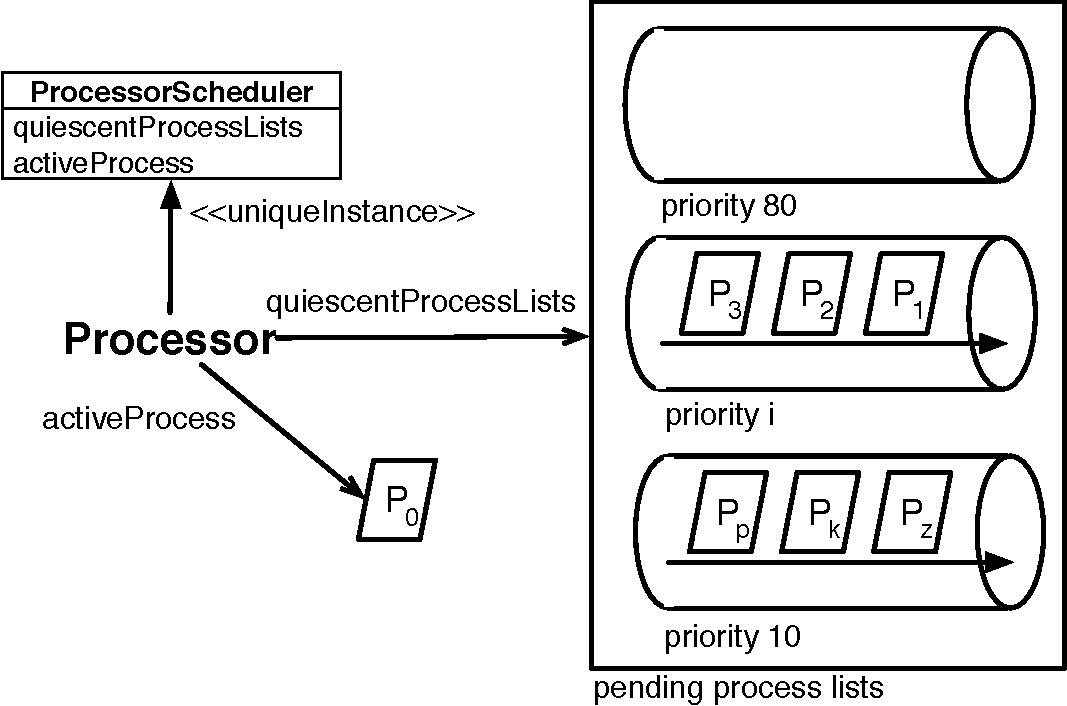
\includegraphics[width=0.6\textwidth]{/Users/ducasse/Workspace/FirstCircle/MyBooks/Bk-Writing/PharoBooks2/Booklet-ConcurrentProgramming/_result/pdf/Chapters/figures/SchedulerSimple.pdf}\caption{The scheduler knows the currently active process as well as the lists of pending processes based on their priority.\label{SchedulerSimple}}\end{center}
\end{figure}


There are simple rules to interrupt and change the process to be run:

\begin{itemize}
\item Processes with higher priority can interrupt lower priority processes if they have to be executed. 
\end{itemize}

\begin{itemize}
\item Processes with the same priority are executed in the same order they were added to scheduled process list.
\end{itemize}

\begin{itemize}
\item As mentioned before, a process (green thread) should use \textcode{Processor yield} to give an opportunity to run to the other processes with the same priority. In this case, the  yielding process is moved to the end of the list to give a chance to execute all the pending processes (see below Scheduler's principles).
\end{itemize}

\begin{note}
In the case of a higher priority level process interrupting a process of lower priority, when the interrupting process releases the control, the question is then what is the next process to resume: the interrupted one or another one. In Pharo legacy, the interrupted process is put at the end of the waiting queue, while a better design is to resume the interrupted process to give it a chance to continue its tasks.
\end{note}
\section{Process}
A process is an instance of the class \textcode{Process}. 
This is class is a subclass of the class \textcode{Link}. 
A link is an element of a linked list (class \textcode{LinkedList}). 
This design is to make sure that processes can be elements in a linked list without wrapping them in a \textcode{Link} instance. 
Note that this linked list is tailored for the Process scheduler logic. 
Better use another one if you need one.

A process has the following instance variables:

\begin{itemize}
\item priority: holds an integer to represent the priority level of the process.
\item suspendedContext: holds the execution context (stack reification) at the moment of the suspension of the process.
\item myList: the list of processes to which the suspended process belongs to. 
\end{itemize}
\section{Conclusion}
We presented briefly the concurrency model of Pharo: preemptive and collaborative. A process of higher priority can stop the execution of processes of lower ones. 
Processes at the same priority should explicit return control using the \textcode{yield} message.
We presented the notion of process (green thread) and process scheduler. 
In the next chapter we explain semaphores since we will explain how the scheduler uses delays to performing its scheduling. 
\chapter{Semaphores}
Often we encounter situations where we need to synchronize processes.
For example, imagine that you only have one pen and that there are several writers wanting to use it.
You will wait for the pen and once the pen is released, you will be able to access and use it.
Now since multiple people can wait for the pen, the waiters are ordered in a waiting list associated with the pen.
When the current writer does not need the pen anymore, he will say it and the next writer in the queue will be able to use it.
Writers needed to use the pen just register to the pen: they are added at the end of the waiting list.

In fact, our pen is a semaphore. Semaphores are the basic bricks for concurrent programming and even the scheduler itself.
\section{Understanding semaphores}
A Semaphore is an object used to synchronize multiple processes.
A semaphore is often used to make sure that a resource is only be accessed by a single process at the time.

A process that wants to access to a resource will declare to the semaphore protecting the resource by sending
to the semaphore the message \textcode{wait}. 
The semaphore will add this process to its waiting list. 
A semaphore keeps a list of waiting processes that want to access to the resource protected by the semaphore.
When the process currently using the resource does not use it anymore, it signals it to the semaphore sending the message \textcode{signal}. 
The semaphore resumes the first waiting process which is added to the suspended list of the scheduler.

Here are the steps:

\begin{enumerate}
\item The semaphore protects resources: P0 is using the ressources, P1...2 are waiting for the resources (Fig. \ref{Sema1}).
\item The process P4 wants to access the resources: it sends wait to the semaphore (Fig. \ref{Sema2}).
\item P4 is added to the waiting list (Fig. \ref{Sema3}).
\item P0 has finished to use the resources: it signals it to the semaphore  (Fig. \ref{Sema4})..
\item The semaphore resumes the first waiting process (P1) (Fig. \ref{Sema5}).
\item The resumed process is now scheduled by the scheduler  (Fig. \ref{Sema6}).
\end{enumerate}


\begin{figure}

\begin{center}
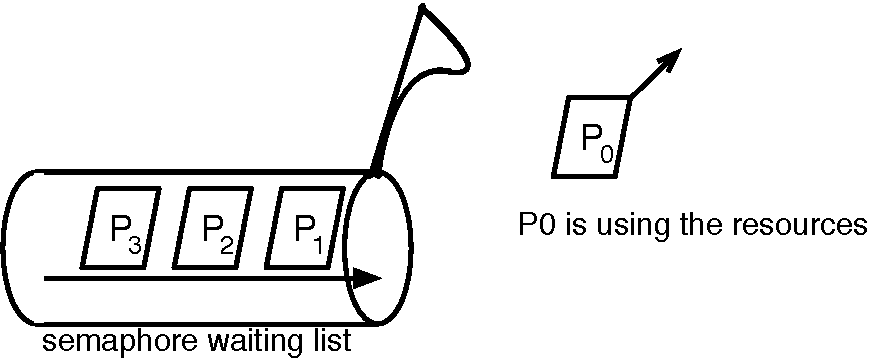
\includegraphics[width=0.6\textwidth]{/Users/ducasse/Workspace/FirstCircle/MyBooks/Bk-Writing/PharoBooks2/Booklet-ConcurrentProgramming/_result/pdf/Chapters/figures/Semaphores1.pdf}\caption{The semaphore protects resources: P0 is using the ressources, P1...2 are waiting for the resources. \label{Sema1}}\end{center}
\end{figure}



\begin{figure}

\begin{center}
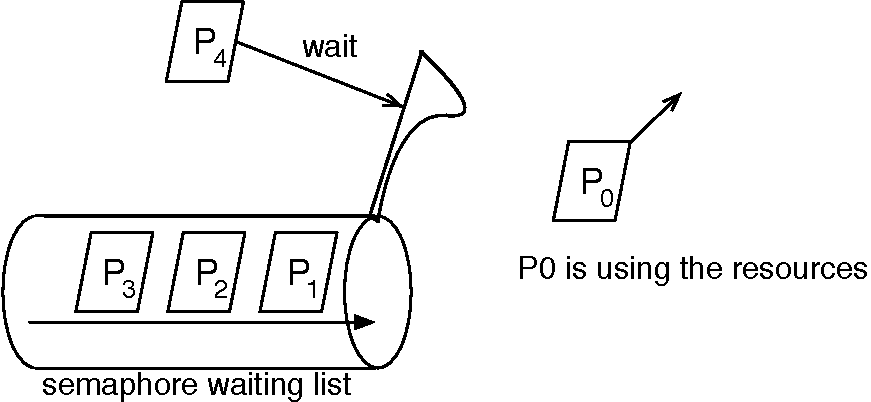
\includegraphics[width=0.6\textwidth]{/Users/ducasse/Workspace/FirstCircle/MyBooks/Bk-Writing/PharoBooks2/Booklet-ConcurrentProgramming/_result/pdf/Chapters/figures/Semaphores2.pdf}\caption{The process P4 wants to access the resources: it sends wait to the semaphore.\label{Sema2}}\end{center}
\end{figure}



\begin{figure}

\begin{center}
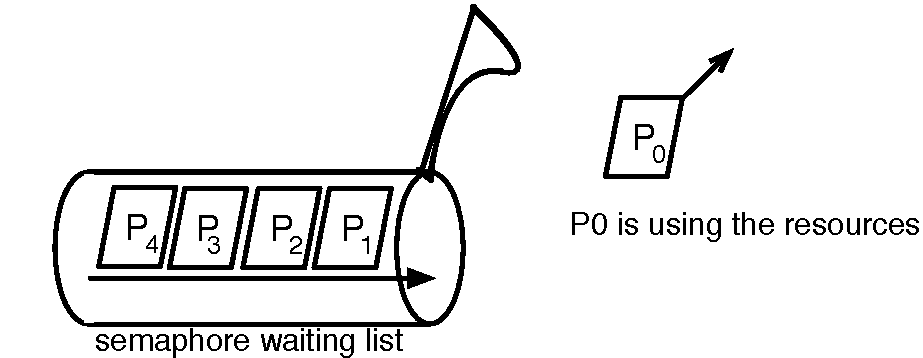
\includegraphics[width=0.6\textwidth]{/Users/ducasse/Workspace/FirstCircle/MyBooks/Bk-Writing/PharoBooks2/Booklet-ConcurrentProgramming/_result/pdf/Chapters/figures/Semaphores3.pdf}\caption{P4 is added to the waiting list.\label{Sema3}}\end{center}
\end{figure}



\begin{figure}

\begin{center}
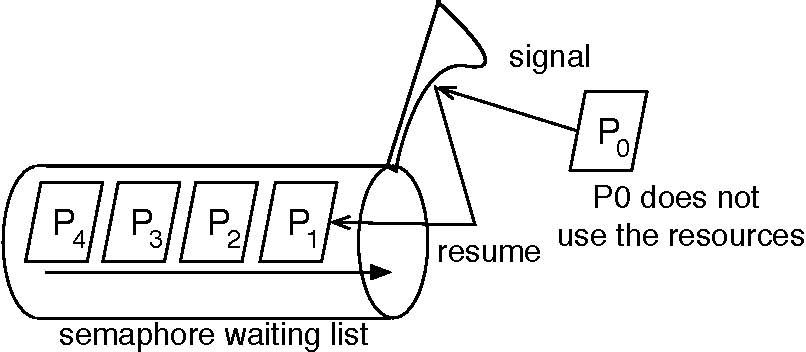
\includegraphics[width=0.6\textwidth]{/Users/ducasse/Workspace/FirstCircle/MyBooks/Bk-Writing/PharoBooks2/Booklet-ConcurrentProgramming/_result/pdf/Chapters/figures/Semaphores4.pdf}\caption{P0 has finished to use the resources: it signals it to the semaphore.\label{Sema4}}\end{center}
\end{figure}



\begin{figure}

\begin{center}
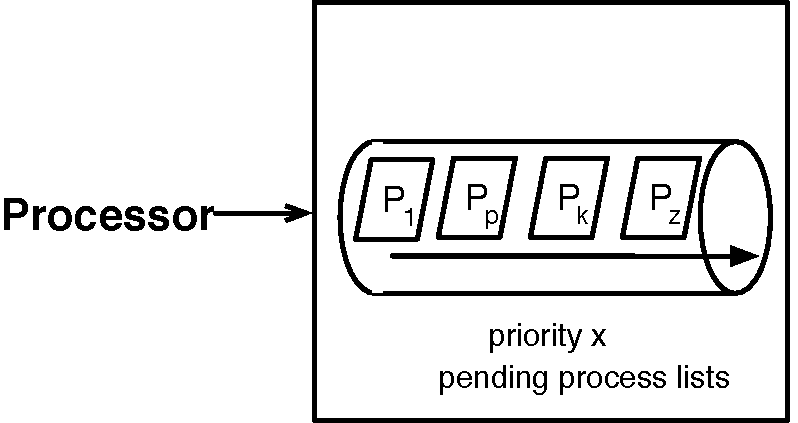
\includegraphics[width=0.6\textwidth]{/Users/ducasse/Workspace/FirstCircle/MyBooks/Bk-Writing/PharoBooks2/Booklet-ConcurrentProgramming/_result/pdf/Chapters/figures/Semaphores5.pdf}\caption{The semaphore resumes the first waiting process (P1).\label{Sema5}}\end{center}
\end{figure}



\begin{figure}

\begin{center}
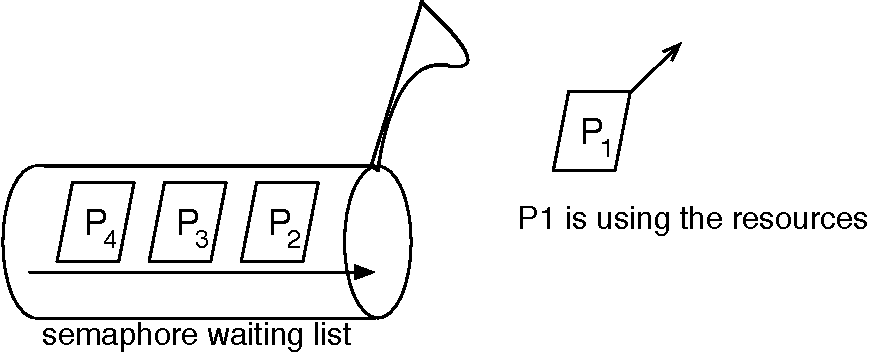
\includegraphics[width=0.6\textwidth]{/Users/ducasse/Workspace/FirstCircle/MyBooks/Bk-Writing/PharoBooks2/Booklet-ConcurrentProgramming/_result/pdf/Chapters/figures/Semaphores6.pdf}\caption{The resumed process is now scheduled by the scheduler.\label{Sema6}}\end{center}
\end{figure}


A semaphore will only release as many processes from \textcode{wait} messages as it has received signal messages.
When a semaphore receives a \textcode{wait} message for which no corresponding \textcode{signal} has been sent, the process sending the \textcode{wait} is suspended.
Each semaphore maintains a linked-list of suspended processes, and releases them on a first–in first–out basis.

Unlike the \textcode{ProcessorScheduler}, a semaphore does not pay attention to the priority of a
\textcode{Process}, it dequeues processes in the order in which they waited on the semaphore.

The dequeued process is resumed and as such it is added in the waiting list of the scheduler.
\section{An example}
Open a transcript and inspect the following piece of code: It schedules two processes and make them both waiting for a semaphore. 

\begin{displaycode}{plain}
| semaphore |
semaphore := Semaphore new.

[ "Do a first job ..."
	'Job1 started' crLog.
	semaphore wait. 
	'Job1 finished' crLog
	] fork.

[ "Do a second job ..."
	'Job2 started' crLog.
	semaphore wait. 
	'Job2 finished' crLog
	] fork.
semaphore inspect
\end{displaycode}

You should see in the transcript the following:

\begin{displaycode}{plain}
'Job1 started'
'Job2 started'
\end{displaycode}

What you see is that the two processes stopped. They did not finish their job. 
When a semaphore receives a \textcode{wait} message, it will stop the process sending the message and add the process to its pending list. 

Now in the inspector on the semaphore execute \textcode{self signal}.
This will have as effect to schedule one of the waiting process and one of the job will finish its task.
\section{Example: Prearmed Semaphore}
Let us modify slightly the previous example. 
We send a \textcode{signal} message to the semaphore prior to creating the processes.

\begin{displaycode}{plain}
| semaphore |
semaphore := Semaphore new.
semaphore signal. 
[ "Do a first job ..."
	'Job1 started' crLog.
	semaphore wait. 
	'Job1 finished' crLog
	] fork.

[ "Do a second job ..."
	'Job2 started' crLog.
	semaphore wait. 
	'Job2 finished' crLog
	] fork.
semaphore
\end{displaycode}

What you see here is that one of the waiting process is proceed.

\begin{displaycode}{plain}
'Job1 started'
'Job1 finished'
'Job2 started'
\end{displaycode}

This example illustrates that a semaphore a \textcode{signal} does not have to be done after a \textcode{wait}.
This is important to make sure that one certain concurrency synchronisation, all the processes are waiting, while the first one could do its task and send a signal to schedule another one. 

A semaphore holds a counter of signals that it receives but did not lead to a process execution, and it will not block the process sending a \textcode{wait} message if it has got  \textcode{signal} messages that did not led to scheduling a waiting process.
\section{Pharo implementation }
A semaphore keeps a number of excess signals: the amount of signals that did not led to schedule a waiting process.

If the number of waiting process on a semaphore is smaller than the number allowed to wait, sending a \textcode{wait} message is not blocking and the process can continue its operations. On the contrary, the process is stored at the end of the pending list and we will scheduled when the previously pending process will be executed. 

Here is the implemntation of \textcode{signal} and \textcode{wait} in Pharo.

The signal message comment shows that if there is no waiting process, the excess signal is increased, else when there are waiting processes, the first one is scheduled.

\begin{displaycode}{plain}
Semaphore >> signal
	"Primitive. Send a signal through the receiver. If one or more processes 
	have been suspended trying to receive a signal, allow the first one to 
	proceed. If no process is waiting, remember the excess signal."

	<primitive: 85>
	self primitiveFailed

	"self isEmpty    
		ifTrue: [excessSignals := excessSignals+1]    
		ifFalse: [Processor resume: self removeFirstLink]"
\end{displaycode}

The description of the wait primitive shows that when a semaphore has some signals on excess, waiting is not blocking, it just decreases the number of signals on excess. 
On the contrary, when there is no signals on excess, then the process is suspended.

\begin{displaycode}{plain}
Semaphore >> wait
	"Primitive. The active Process must receive a signal through the receiver 
	before proceeding. If no signal has been sent, the active Process will be 
	suspended until one is sent."

	<primitive: 86>
	self primitiveFailed

	"excessSignals>0  
		ifTrue: [excessSignals := excessSignals-1]  
		ifFalse: [self addLastLink: Processor activeProcess suspend]"
\end{displaycode}
\section{wait and signal interplay}
The following example schedule three processes. It shows that thread can wait, do some action, signal that they are done that other threads in reaction can get scheduled.

\begin{displaycode}{plain}
| semaphore |
semaphore := Semaphore new. 
[ 'Pharo ' crLog ] fork. 

['is ' crLog .
semaphore wait.
'super ' crLog. 
semaphore signal] fork.

['really ' crLog. 
semaphore signal.
semaphore wait.
'cool!' crLog ] fork
\end{displaycode}

You should obtain \textcode{Pharo is really super cool!}

Let us describe what is happening. 

\begin{itemize}
\item The first one prints \textcode{'Pharo'}. 
\item The second one prints \textcode{'is '} and waits.
\item The third one prints \textcode{'really '} and signal the semaphore and waits. It is added to the waiting list after the second process.
\item Since the third process signaled the semaphore, the first waiting process (the second one) is scheduled and prints \textcode{'super '} and signals the semaphore. 
\item The third process is scheduled and prints: \textcode{'cool!'}
\end{itemize}
\chapter{Scheduler's principles}
Un processus signifie \`{a} un s\'{e}maphore qu’il lib\`{e}re la ressource en lui envoyant le message signal. 
Le s\'{e}maphore envoie alors un message resume au premier processus en attente de sa file d’attente, 
ce qui rend ce dernier activable, c’est-\`{a}-dire qu’il est ajout\'{e} dans la file d’attente du 
ProcessorScheduler correspondant \`{a} sa priorit\'{e} (voir figure 9-2 ci-apr\`{e}s).


\begin{figure}

\begin{center}
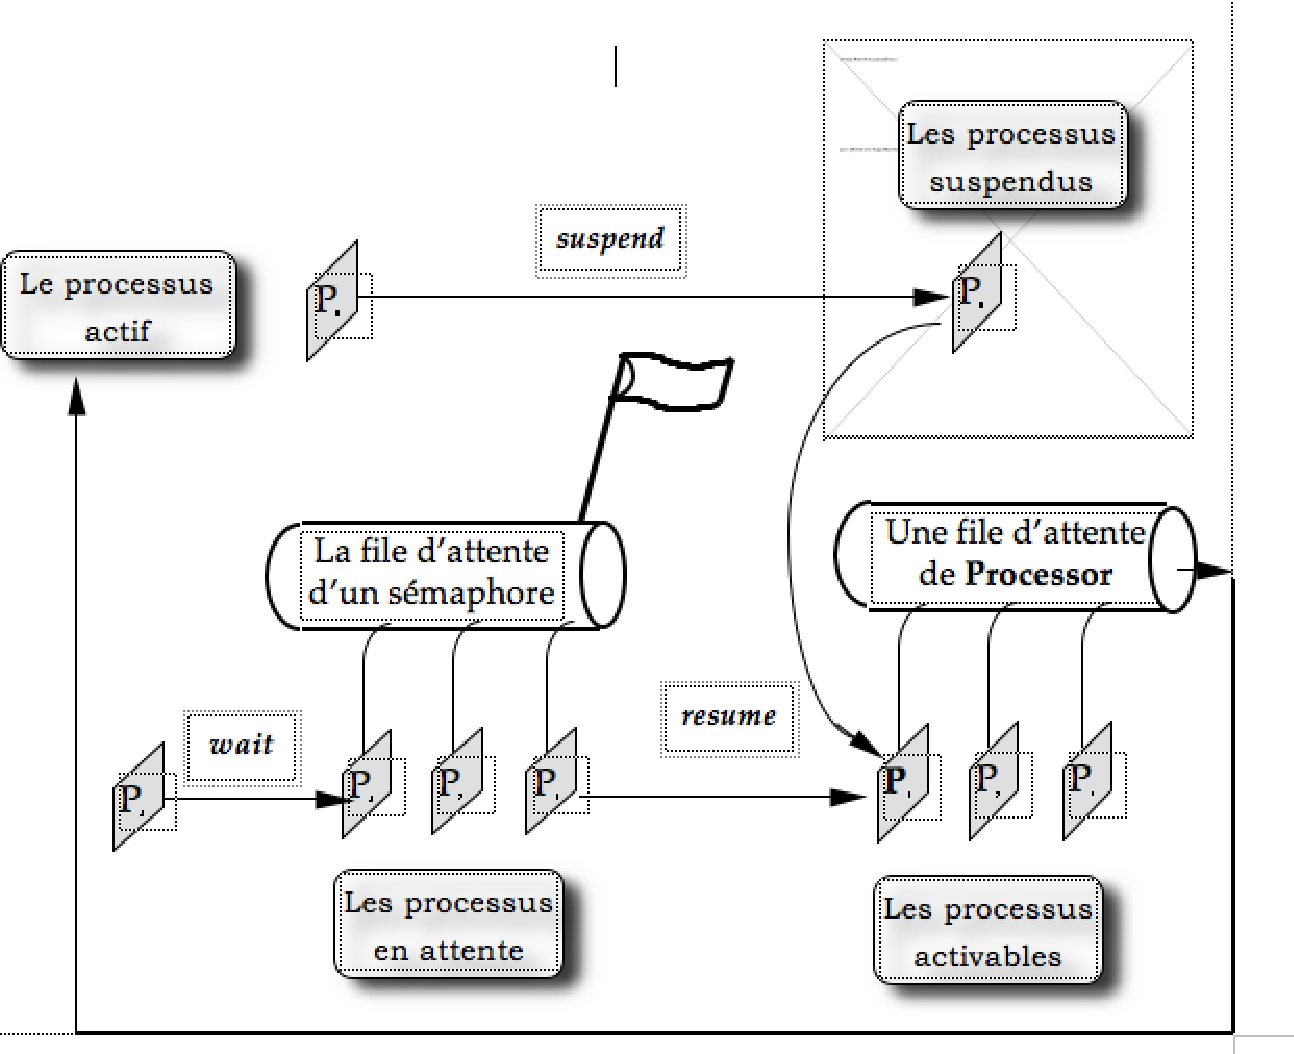
\includegraphics[width=1.0\textwidth]{/Users/ducasse/Workspace/FirstCircle/MyBooks/Bk-Writing/PharoBooks2/Booklet-ConcurrentProgramming/_result/pdf/Chapters/figures/ProcessorStateSchedulerSemaphore.pdf}\caption{BBB\label{ProcessorStateSchedulerSemaphore}}\end{center}
\end{figure}


Now we can revisit the different states of a process by looking its interaction with the process scheduler and 
semaphores as shown in \ref{ProcessorStateScheduler}.

\begin{itemize}
\item active: it is currently executed.
\item activable: it is one of the waiting queue of the scheduler.
\item waiting: it is suspendedn on a semaphore. It is the waiting list of a semaphore and it is not yet activable.
\item suspended: if this is the active process it is interrupted and can be reactivated later, else it is removed from the queue of the activable process that it belongs to. 
\end{itemize}


\begin{figure}

\begin{center}
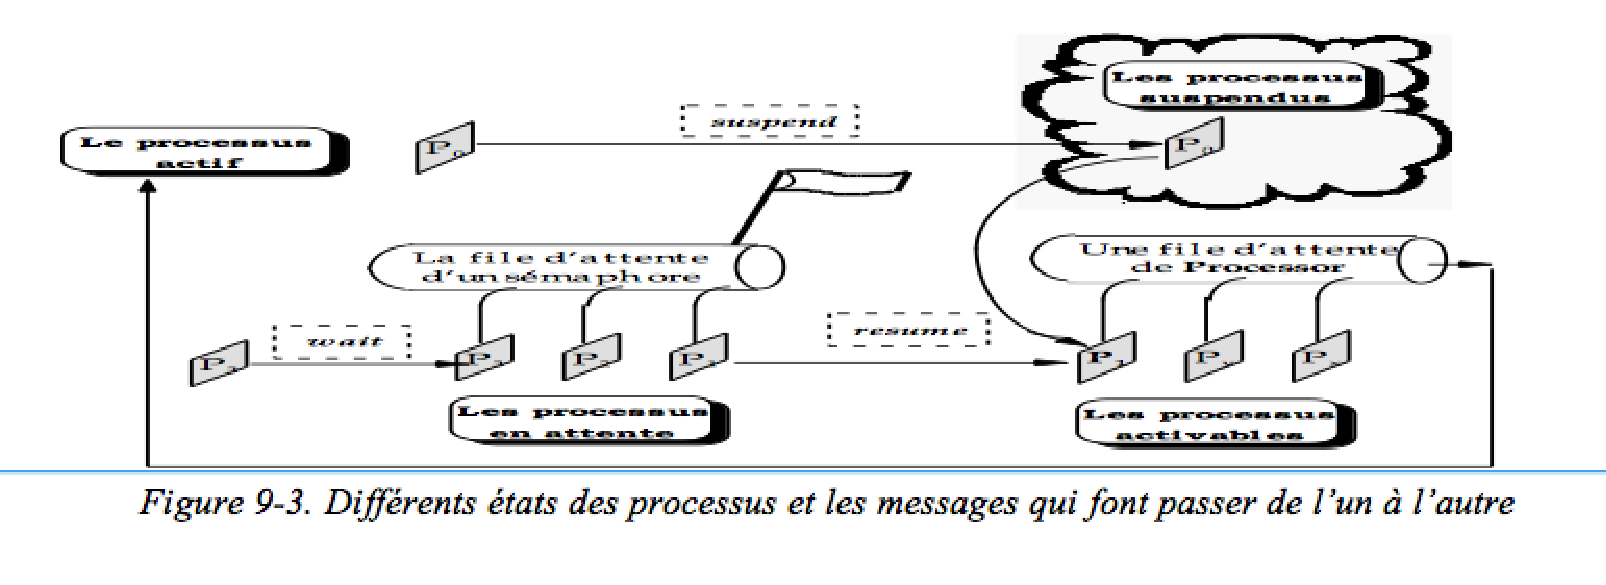
\includegraphics[width=1.0\textwidth]{/Users/ducasse/Workspace/FirstCircle/MyBooks/Bk-Writing/PharoBooks2/Booklet-ConcurrentProgramming/_result/pdf/Chapters/figures/ProcessorStateScheduler.pdf}\caption{Revisiting the process states\label{ProcessorStateScheduler}}\end{center}
\end{figure}

\section{Delay}
In case you need to pause execution for some time, you can use \textbf{Delay}.

Delays can be instantiated and set up by sending \textcode{forSeconds:} or \textcode{forMilliseconds:} to the class \textcode{Delay} and executed by sending it \textcode{wait} message.

For example:

\begin{displaycode}{plain}
| delay |
delay := Delay forSeconds: 3.
[ 1 to: 10 do: [:i |
  Transcript show: i printString ; cr.
  delay wait ] ] fork
\end{displaycode}

will print a number each 3 seconds.

Delays suspend the execution of a thread during a precise duration. The thread is then in suspended state.

Typical needs for delas are 

\begin{itemize}
\item repeat an action every x milliseconds.
\item wait a given amount of time before executing an action. 
\end{itemize}
\section{Example}
\begin{displaycode}{plain}
[
| betweenPing |  
betweenPing := Delay forMilliseconds: 300.
10 timesRepeat: [ 
   'ping' crLog. 
   betweenPing wait] 
   ] forkAt: Processor userBackgroundPriority.
	  
[
| betweenPong |  
betweenPong := Delay forMilliseconds: 100.
10 timesRepeat: [ 
   'PONG' crLog. 
   betweenPong wait]
   ] forkAt: Processor userBackgroundPriority.
\end{displaycode}
\chapter{Synchronisation}
When multiple threads share and modify the same resources we can easily end up in 
broken state. 
\section{Motivation}
Let us imagine that two threads are accessing an account to redraw money.
When the threads are not synchronised you may end up to the following situation
that one thread access information while the other thread is actually modifying. 

Here we see that we redraw 1000 and 200 but since the thread B reads before 
the other thread finished to commit its changes, we got desynchronised.

\begin{tabular}{lll}
\toprule
\textbf{Thread A: account debit: 1000} & \textbf{Thread B: account debit: 200} &  \\
\midrule
Reading: account value -\textgreater{} 3000 &  &  \\
account debit: 1000 & Reading: account value = 3000 &  \\
account value -\textgreater{} 2000 & account debit: 200 &  \\
 & account value -\textgreater{} 2800 \\
\bottomrule
\end{tabular}

The solution is to make sure that a thread cannot access a resources while another one is modifying it. Basically we want that all the threads sharing a resources are mutually exclusive. 

When several access a shared resources, only one gets the resources, the other threads got suspended, waiting for the first thread to have finished and release the resources.
\section{Using a semaphore}
We can use a semaphore to control the execution of several threads. 

Here we want to make sure that we can do 10 debit and 10 deposit of the same amount and that we get the same amount at the end. 

\begin{displaycode}{plain}
|lock account|
lock := Semaphore new.
account := 3000.
[ 10 timesRepeat: [
	lock wait.
	counter := counter + 100.
	compter crLog.
	lock signal ]
	] fork.
	
[ 10 timesRepeat: [
	counter := counter - 100.
	counter crLog. 
	lock signal. 
	lock wait ]
	] fork
\end{displaycode}

Notice the pattern, the thread are not symmetrical. 
The first one will first wait that the resources is accessible and perform his work 
and signals that he finished. 
The second one will work and signal and wait to perform the next iteration.

The same problem can be solved in a more robust wait using Mutex and critical sections
as we see present in the following section.
\section{Using a Mutex}
A Mutex is an object to protect a share resources. An instance of the class \textcode{Mutex} will make sure that only one thread of control can be executed simultaneously on a given portion of code using the message \textcode{critical:}.

In the following example the expressions \textcode{Processor yield} ensures that thread of the same priority can get a chance to be executed. 

\begin{displaycode}{plain}
|lock account|
lock := Mutex new.
account := 3000.
[10 timesRepeat: [ Processor yield.
	lock critical: [ account := counter + 100.
					account crLog ] ]
	] fork.

[10 timesRepeat: [ Processor yield.
	lock critical: [ account := counter - 100.
					account crLog ] ]
	] fork
\end{displaycode}
\section{Shared Queue}
Instances de la classe SharedQueue  –  Canaux d'échange d'objets 
•  Analogues aux sockets/streams ou pipes unix  –  Mais, synchronisés 
•  1 écrivain ou 1 lecteur à la fois 
•  Les lecteurs sont bloqués quand la file est vide

\begin{displaycode}{plain}
|file| 
file := SharedQueue new.
[
	[ |number| "reader 1"
	number := file next.
	number ifNil: [Processor terminateActive].
	number crLog ] repeat
	] fork. 
\end{displaycode}

\begin{displaycode}{plain}
	[ |counter| "reader 2" 
	counter := 0. 
	[file next ifNil: [ ('total = ', counter asString) crLog.
		Processor terminateAc3ve].
		counter := counter + 1 ] repeat 
	] fork.
\end{displaycode}

 {[}{[}{[}
{[}	
	\textbar{}delayBetweenWrite\textbar{}
	delayBetweenWrite := Delay forMilliseconds: 100.   
	1 to: 10 do: {[}:numb\textbar{} 
		delayBetweenWrite wait.
		file nextPut: numb{]}.
	2 timesRepeat: {[}file nextPut: nil{]}
	{]} fork. 
{]}{]}{]}
\chapter{Monitor}
A monitor provides process synchronization that is more high-level than the one provided by a semaphore. A monitor has the following properties:

\begin{enumerate}
\item At any time, only one process can execute code inside a critical section of a monitor.
\item A monitor is reentrant, which means that the active process in a monitor never gets blocked when it enters a (nested) critical section of the same monitor.
\item Inside a critical section, a process can wait for an event that may be coupled to a certain condition. If the condition is not fulfilled, the process leaves the monitor temporarily (to let other processes enter) and waits until another process signals the event. Then, the original process checks the condition again (this is often necessary because the state of the monitor could have changed in the meantime) and continues if it is fulfilled.
\item The monitor is fair, which means that the process that is waiting on a signaled condition the longest gets activated first.
\item The monitor allows you to define timeouts after which a process gets activated automatically.
\end{enumerate}
\section{Basic usage:}
Monitor\textgreater{}\textgreater{}critical: aBlock
Critical section.
Executes aBlock as a critical section. At any time, only one process can execute code in a critical section.
NOTE: All the following synchronization operations are only valid inside the critical section of the monitor!

Monitor\textgreater{}\textgreater{}wait
Unconditional waiting for the default event.
The current process gets blocked and leaves the monitor, which means that the monitor allows another process to execute critical code. When the default event is signaled, the original process is resumed.

Monitor\textgreater{}\textgreater{}waitWhile: aBlock
Conditional waiting for the default event.
The current process gets blocked and leaves the monitor only if the argument block evaluates to true. This means that another process can enter the monitor. When the default event is signaled, the original process is resumed, which means that the condition (argument block) is checked again. Only if it evaluates to false, does execution proceed. Otherwise, the process gets blocked and leaves the monitor again...

Monitor\textgreater{}\textgreater{}waitUntil: aBlock
Conditional waiting for the default event.
See Monitor\textgreater{}\textgreater{}waitWhile: aBlock.

Monitor\textgreater{}\textgreater{}signal
One process waiting for the default event is woken up.

Monitor\textgreater{}\textgreater{}signalAll
All processes waiting for the default event are woken up.
\section{We need one example here}\chapter{Mutex implementation}
I would love to understand it :)
\chapter{ShareQueue: a Semaphore Example}
\begin{todo}
translate stef! 
\end{todo}

Une SharedQueue, ou file partag\'{e}e, est une structure FIFO (First In First Out, le premier \'{e}l\'{e}ment entr\'{e} est le premier sorti), dot\'{e}e de s\'{e}maphores de protection contre les acc\`{e}s concurrents. Cette structure est utilis\'{e}e dans les situations o\`{u} plusieurs processus fonctionnent simultan\'{e}ment et sont susceptibles d’acc\'{e}der \`{a} cette m\^{e}me structure.
Sa d\'{e}finition est la suivante :

\begin{displaycode}{plain}
Object subclass: #SharedQueue
	instanceVariableNames: 'contentsArray readPosition writePosition accessProtect readSynch ' 
	package: 'Collections-Sequenceable'
\end{displaycode}

\textcode{accessProtect} est un s\'{e}maphore d’exclusion mutuelle pour l’\'{e}criture, tandis que readSync est utilis\'{e} pour la synchronisation en lecture. Ces variables sont instanci\'{e}es par la m\'{e}thode d’initialisation de la fa\c{c}on suivante :

\begin{displaycode}{plain}
accessProtect := Semaphore forMutualExclusion.
readSynch := Semaphore new
\end{displaycode}

Ces deux s\'{e}maphores sont utilis\'{e}s dans les m\'{e}thodes d’acc\`{e}s et d’ajouts d’\'{e}l\'{e}ments (voir figure 6- 5).

\begin{displaycode}{plain}
SharedQueue >> next
	| value |
	readSynch wait.
	accessProtect
		critical: [readPosition = writePosition
				ifTrue: [self error: 'Error in SharedQueue synchronization'.
					Value := nil]
				ifFalse: [value := contentsArray at: readPosition.
					contentsArray at: readPosition put: nil.
					readPosition := readPosition + 1]].
	^ value
\end{displaycode}

Dans la m\'{e}thode d’acc\`{e}s, next, le s\'{e}maphore de synchronisation en lecture « garde » l’entr\'{e}e de la m\'{e}thode (ligne 3). Si un processus envoie le message next alors que la file est vide, il sera suspendu et plac\'{e} dans la file d’attente du s\'{e}maphore readSync par la m\'{e}thode wait. Seul l’ajout d’un nouvel \'{e}l\'{e}ment pourra le rendre \`{a} nouveau actif. La section critique g\'{e}r\'{e}e par le s\'{e}maphore accessProtect (lignes 4 \`{a} 10) garantit que la portion de code contenue dans le bloc est ex\'{e}cut\'{e}e sans qu’elle puisse \^{e}tre interrompue par un autre s\'{e}maphore, ce qui rendrait l’\'{e}tat de la file inconsistant.

Dans la m\'{e}thode d’ajout d’un \'{e}l\'{e}ment, \textcode{nextPut:}, la section critique (lignes 3 \`{a} 6) prot\`{e}ge l’\'{e}criture, apr\`{e}s laquelle le s\'{e}maphore \textcode{readSync} est \textit{signal\'{e}e}, ce qui rendra actif les processus en attente de donn\'{e}es.

\begin{displaycode}{plain}
SharedQueue >> nextPut: value 
	accessProtect
		critical: [ writePosition > contentsArray size
				ifTrue: [self makeRoomAtEnd].
			contentsArray at: writePosition put: value.
			WritePosition := writePosition + 1].
			readSynch signal.
			^ value
\end{displaycode}
\section{Conclusion}
We presented the key elements of basic concurrent programming in Pharo and some implementation details.


% lulu requires an empty page at the end. That's why I'm using
% \backmatter here.
\backmatter

% Index would go here

\end{document}
